\section{Transport of concentrate}\label{se:transport_of_concentrate}

A model for transport of concentrate in sewer pipes is obtained in the following.
The following assumptions are made obtaining the transport equation.

 \begin{table}[H]
\begin{enumerate}
	\item The flow of concentrate is assumed to be steady and uniform in the cross section.
	\item The anoxic, anaerobic or aerobic processes occurring in the sewer line is neglected   
\end{enumerate}
\label{tab:concentrate_flow}
\end{table}
 
In figure \ref{fig:poopvolume} a control volume is seen.
\begin{figure}[H]
\centering
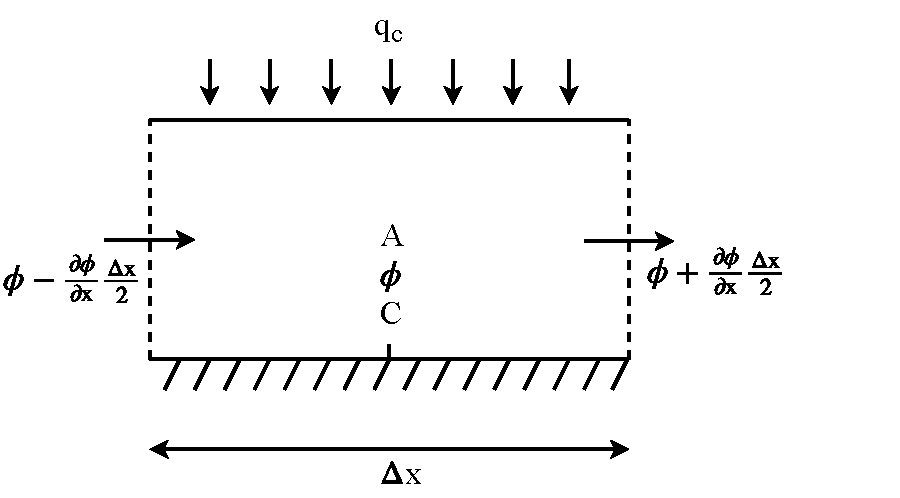
\includegraphics[width=.8\textwidth]{report/modeling/pictures/poopvolume.pdf}
\caption{Illustration of a control volume containing concentrate.}
\label{fig:poopvolume}
\end{figure} 

The conservation of concentrate in the control volume is as in section \ref{se:hydraulics_of_sewer_line} dependent on the change in stored mass and change in flow. This means that the equation for conservation of mass given by equation \ref{saintbernard_mass_lateral}, which is shown below, can be utilized.

\begin{equation}	
\frac{\partial A}{\partial t} + \frac{\partial Q}{\partial x}=q
\label{eq:saintbernard_continuity_conflow}
\end{equation}

Assuming average concentrate, C, across the control volume, and multiplying it with the terms of the continuity equation, the following is obtained:
%Assuming average concentrate, C, across the control volume, and multiplying it with the time derivative and lateral inflow term and replacing the flow term, Q, with a flux term, the following is obtained:
%Multiplying the terms of the continuity equation with the concentrate yields the following:
\begin{equation}
%\begin{array}{l}
%	\frac{\partial A \cdot C}{\partial t} + \frac{\partial Q}{\partial x}=q \cdot C \\
%	\updownarrow \\
	\frac{\partial A \cdot C}{\partial t} + \frac{\partial \phi}{\partial x}=q \cdot C_{lat} \\
%\end{array}	
\label{poop_mass_equation}
\end{equation}
 % A derivation of a one dimensional model for transport of concentration, in channel flow, is given. 
 % As in section \ref{se:hydraulics_of_sewer_line} certain assumptions is made when deriving the model.



% %  \begin{figure}[H]
% % \centering
% % 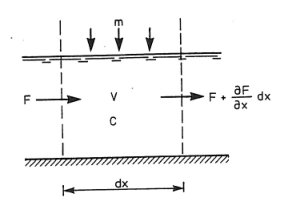
\includegraphics[width=.6\textwidth]{report/modeling/pictures/concentrate_volume.png}
% % \caption{Illustration of a control volume with concentrate.}
% % \label{fig:concentrate_volume}
% % \end{figure} 

% From the control volume an equation for conservation of continuity can be derived as in section \ref{se:hydraulics_of_sewer_line}. The change of stored concentrate in the control volume is given as:

% \begin{equation}
%  \left(V \cdot C + \frac{\partial (V\cdot C)}{\partial t} \frac{\Delta x}{2} \Delta t \right) - \left(V \cdot C - \frac{\partial (V\cdot C)}{\partial t} \Delta t \right) = \frac{\partial (V\cdot C)}{\partial t}\Delta t
% \label{eq:poop_storing}
% \end{equation}

% Where V is the volume [$m^3$] and C is the concentrate [$\frac{g}{m^3}$]. 

% The flux of concentrate in and out of the control volume at a given time $\Delta t$ is given as:


%  \begin{equation}
%   	\left( \phi_{in} - \phi_{out} + \phi_{lateral} \right) \Delta t   =	\phi \cdot \Delta t - \left(\phi + \frac{\partial \phi}{\partial x}\Delta x \right) \Delta t + m \cdot \Delta x \cdot \Delta t = - \frac{\partial \phi}{\partial x}\cdot \Delta x \cdot \Delta t +m \cdot \Delta x \cdot \Delta t  
%   \label{eq:poop_flux_in_out}
%   \end{equation} 

Where $\phi$ is a flux [$\frac{g}{s}$] term replacing the flow term, $Q$ and $C_{lat}$ is lateral concentrate input into the control volume [$\frac{g}{m^3}$] \cite{vestergaard1989numerical}.

%The continuity equation can now be stated as the change in stored concentration equal to the sum of flux in- and outflow from the control volume as given by equation \ref{eq:poop_storing} and \ref{eq:poop_flux_in_out}:

% \begin{equation}
% 	\frac{\partial (V\cdot C)}{\partial t}\Delta t = - \frac{\partial \phi}{\partial x}\cdot \Delta x \cdot \Delta t +m \cdot \Delta x \cdot \Delta t
% \end{equation}

% When replacing V with $\text{A}\cdot \Delta \text{x}$ and dividing with $\Delta x \cdot  \Delta t$ then the basic continuity equation of conservation is obtained:

% \begin{equation}
% 	\frac{\partial (A\cdot C)}{\partial t} = - \frac{\partial \phi}{\partial x} + q_c 
% \label{eq:concentrate_continuity_equation}
% \end{equation}

Depending on the desired approximation the flux and lateral inflow terms can be expanded. The expanded lateral term describes a dead zone at the bottom of the channel, which can be useful to model if dealing with rugged channel bed. Due to the prismatic assumption in section \ref{se:hydraulics_of_sewer_line} of the sewer channel the dead zone in the channel is not investigated further. Flux terms describing convective flow and dispersion can be seen in table \ref{tab:flux_terms}.  

\begin{table}[H]
\centering
	\begin{tabular}{|l|l|l|} \hline
	\rowcolor[HTML]{9B9B9B} 
	\textbf{Approximation} 	& \textbf{Convective flow} &	\textbf{Convective + (dispersion)}  \\ \hline
	Flux term   	& $\phi = Q \cdot C$ & $ \phi = Q \cdot C + \left(- \epsilon \cdot A \frac{\partial C}{\partial x} \right)$  \\ \hline
	boundary conditions &\multirow{2}{*} 1 &\multirow{2}{*} 2 \\ 
	required			& & \\ \hline
  	\end{tabular} 
\caption{Table of convective flux term without and with dispersion where Q is flow, C is concentrate, A is area and $\epsilon$ is a dispersion coefficient [$\frac{m^2}{s}$] \cite{vestergaard1989numerical} .}
\label{tab:flux_terms} 
\end{table}

The dispersion term shown in the above table, also known as Fickian diffusion, gives an expression for how the molecules of the concentrate are spreading. On a molecular level, the concentrate will to some degree disperse upstream and downstream as shown in figure \ref{fig:diffusion_example}. 

\begin{figure}[H]
\centering
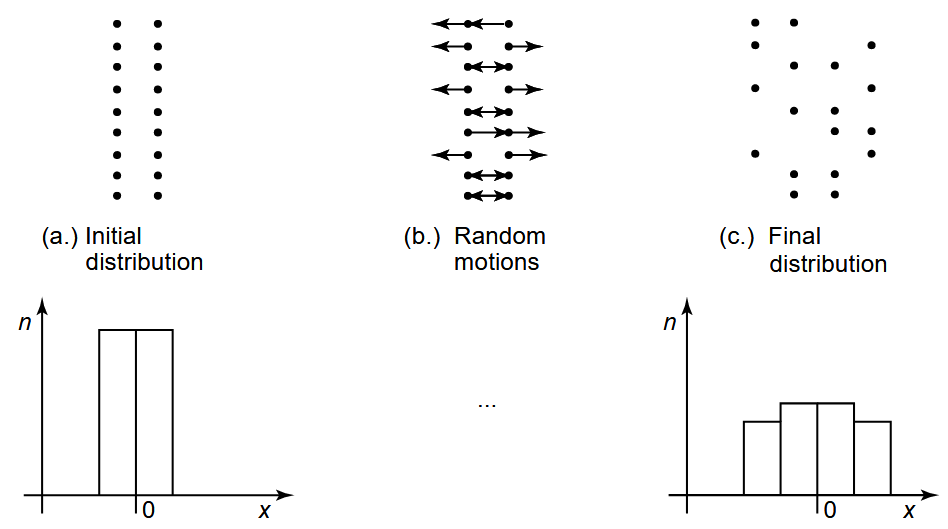
\includegraphics[width=.75\textwidth]{report/modeling/pictures/diffusion_example.png}
\caption{Illustration of distribution of convective flow without dispersion (a) and with (c), where dots illustrate molecules of the concentrate within a control volume \cite{karlruhe_con_def_dif_equation}.}
\label{fig:diffusion_example}
\end{figure} 

For various concentrates the dispersion coefficient $\epsilon$ which varies with temperature can be found in lookup tables \cite{karlruhe_con_def_dif_equation}.

Inserting the terms in table \ref{tab:flux_terms} into equation \ref{poop_mass_equation} then the following expressions of the continuity equation is obtained:

\begin{equation}
	\frac{\partial (A\cdot C)}{\partial t} + \frac{\partial (Q \cdot C)}{\partial x} - \epsilon \cdot \frac{\partial^2 (A \cdot C)}{\partial x^2} = q \cdot C_{lat} 
\label{eq:concentrate_continuity_equation_dispersion}
\end{equation}

\begin{equation}
\frac{\partial (A\cdot C)}{\partial t} + \frac{\partial (Q \cdot C)}{\partial x} = q \cdot C_{lat} 
\label{eq:concentrate_continuity_equation_convective}
\end{equation}

In closed environments such as sewers longitudinal dispersion can often be neglected\cite{vestergaard1989numerical}. For this reason and to reduce complexity of the simulation, equation \ref{eq:concentrate_continuity_equation_convective} is utilized further on.
As the change in flow and area in the channel is solved by the Saint-Venant equations, an expression which only considers a change in concentrate suffices.
The terms in equation \ref{eq:concentrate_continuity_equation_convective} can be rewritten to the following:
\begin{equation}
	C \cdot \frac{\partial A}{\partial t} + A \cdot \frac{\partial C}{\partial t} + C \cdot \frac{\partial Q}{\partial x} + Q \cdot \frac{\partial C}{\partial x} = q \cdot C_{lat}
\label{eq:poop_trans_deriv1}
\end{equation}

Multiplying equation \ref{eq:saintbernard_continuity_conflow} with C yields:
\begin{equation}
	C \cdot \frac{\partial A}{\partial t} + C \cdot \frac{\partial Q}{\partial x} = q \cdot C
	\label{eq:poop_trans_deriv2} 
\end{equation} 

Subtracting equation \ref{eq:poop_trans_deriv2} from \ref{eq:poop_trans_deriv1} then results in the following:

\begin{equation}
	A \cdot \frac{\partial C}{\partial t} + Q \cdot \frac{\partial C}{\partial x} = q \cdot (C_{lat}-C)
	\label{eq:poop_conservation_semi_final} 
\end{equation} 

Neglecting lateral flow and concentration inputs the following expression is obtained:

\begin{equation}
\boxed{	A \cdot \frac{\partial C}{\partial t} + Q \cdot \frac{\partial C}{\partial x} = 0}
	\label{eq:poop_conservation_final} 
\end{equation} 

Equation \ref{eq:poop_conservation_final} can thereby be solved with the solutions of Q and A obtained from the Saint-Venant equations.